% (c) 2012 Tiziana Manca - tmanca@libero.it
% (c) 2012 -2014 Dimitrios Vrettos - d.vrettos@gmail.com
% (c) 2014 Daniele Zambelli - daniele.zambelli@gmail.com
\begin{comment}

\begin{esercizio}
\label{ese:c_stat_}
\end{esercizio}

\end{comment}

\section{Esercizi}

\subsection{Esercizi dei singoli paragrafi}

% \subsubsection*{\numnameref{sec:A_indagine}}

\subsubsection{Tabelle a doppia entrata e indipendenza}

\begin{esercizio}
\label{ese:c_stat_001}
Data la seguente tabella:
\begin{center}
% \begin{tabular}{|p{2.5cm}|p{2cm}|p{2cm}|p{2cm}|p{2.5cm}|}
\setlength{\tabcolsep}{.8cm}
\begin{tabular}{|c|c|c|c|c|}
\hline
$y/x$ & a & b & c & Totale righe\\
\hline
A & 7 & 4 & 1 & \\
\hline
B & 2 & 8 & 3 & \\
\hline
C & 4 & 5 & 9 & \\
\hline
Totale colonne & & & & \\
\hline
\end{tabular}
\end{center}

\begin{enumerate}
\item completa la tabella con le somme parziali e totale
\item scrivere la distribuzione marginale delle $x_i$
\item scrivere la distribuzione marginale delle $y_i$
\item calcolare la media della distribuzione marginale delle $x_i$ 
\hfill $[2]$
\end{enumerate}
\end{esercizio}

\begin{esercizio}
\label{ese:c_stat_002}
Nella seguente tabella sono riportati i dati ottenuti allo scrutinio 
finale di una prima superiore di un gruppo di studenti provenienti da una 
data scuola media e il giudizio conseguito all'esame di licenza:
\begin{center}
\begin{tabular}{|p{1.8cm}|p{1.8cm}|p{2cm}|p{1.8cm}|p{1.8cm}|p{1.8cm}|}
\hline
& ammessi & non ammessi & 1 debito & 2 debiti & 3 debiti\\
\hline
Sufficiente & 0 & 0 & 0 & 0 & 0\\
\hline
Buono & 1 & 0 & 1 & 3 & 5\\
\hline
Distinto & 8 & 1 & 1 & 1 & 0\\
\hline
Ottimo & 15 & 0 & 0 & 0 & 0\\
\hline
\end{tabular}
\end{center}

\begin{enumerate}
\item Determina le distribuzioni marginali dei due 
caratteri:\textquotedblleft Giudizio conseguito all'esame di licenza 
media\textquotedblright e \textquotedblleft risultato ottenuto allo 
scrutinio della fine della prima superiore\textquotedblright
\item Tra gli studenti provenienti da quella scuola media, qual è la 
percentuale di coloro che sono stati promossi senza debito in prima 
superiore? \hfill $[67\%]$
\item Tra gli studenti di quella scuola media che sono stati promossi senza 
debito in prima, qual è la percentuale di coloro che hanno conseguito 
all'esame di licenza un giudizio \textquotedblleft ottimo\textquotedblright 
? \hfill $[62,5\%]$
\item Tra gli studenti di quella scuola media che hanno conseguito 
all'esame di licenza un giudizio \textquotedblleft buono\textquotedblright 
o \textquotedblleft distinto\textquotedblright, qual è la percentuale di 
quelli che sono stati promossi con almeno un debito? \hfill $[52\%]$
\end{enumerate}
\end{esercizio}

\begin{esercizio}
\label{ese:c_stat_003}
Verificare se le variabili $x$ e $y$ delle distribuzioni assegnate 
sono dipendenti o indipendenti:
\begin{center}
\begin{tabular}{|p{1.7cm}|p{1.7cm}|p{1.7cm}|p{1.7cm}|p{2cm}|}
\hline
$y/x$ & a & b & c & Totale righe\\
\hline
A & 3 & 9 & 18 & 30 \\
\hline
B & 5 & 15 & 30 & 50 \\
\hline
C & 6 & 18 & 36 & 60 \\
\hline
Totale & 14 & 42 & 84 & 140 \\
\hline
\end{tabular}
\end{center}

\hfill $[indipendenti]$
\end{esercizio}

\begin{esercizio}
\label{ese:c_stat_004}
Verificare se le variabili $x$ e $y$ delle distribuzioni assegnate 
sono dipendenti o indipendenti:
\begin{center}
\begin{tabular}{|p{1.7cm}|p{1.7cm}|p{1.7cm}|p{1.7cm}|p{2cm}|}
\hline
$y/x$ & a & b & c & Totale righe\\
\hline
A & 1 & 8 & 13 & 22 \\
\hline
B & 4 & 6 & 3 & 13 \\
\hline
C & 8 & 12 & 2 & 22 \\
\hline
Totale & 13 & 26 & 18 & 57 \\
\hline
\end{tabular}
\end{center}
\hfill $[dipendenti]$
\end{esercizio}

\begin{esercizio}
\label{ese:c_stat_005}
In una città sono stati osservati giornalmente le condizioni meteo 
($x$) e il livello di traffico ($y$) per un periodo di un anno. I dati 
ricavati sono stati riassunti nella seguente tabella:
\begin{center}
\begin{tabular}{|p{1.7cm}|p{1.7cm}|p{1.7cm}|p{1.7cm}|p{1.7cm}|}
\hline
$x/y$ & Basso & Medio & Alto & Totale\\
\hline
sereno & 80 & 28 & 12 & 120 \\
\hline
variabile & 32 & 92 & 30 & 154 \\
\hline
perturbato & 8 & 25 & 58 & 91 \\
\hline
totale & 120 & 145 & 100 & 365 \\
\hline
\end{tabular}
\end{center}

\begin{enumerate}
 \item calcola l'indice $\chi^2$ \hfill $[152,3]$
 \item mediante la normalizzazione del $\chi^2$, determina una 
percentuale che esprima la misura dell'associazione tra i due caratteri. 
\hfill $[21\%]$
\end{enumerate}
\end{esercizio}

\begin{esercizio}
\label{ese:c_stat_006}
Sono stati intervistati 20 laureati e su ciascuno sono stati rilevati 
congiuntamente due caratteri: il sesso indicato con X (M= maschio, F= 
femmina) e il tempo (in mesi) occorso per trovare lavoro dopo la laurea, 
indicato con Y (6,12,18,24, mesi).
\begin{center}
\begin{tabular}{ccccccccccc}
\toprule
N° ordine & 1 & 2 & 3 & 4 & 5 & 6 & 7 & 8 & 9 & 10 \\
X & M & M & F & M & M & F & F & F & M & F \\
Y & 6 & 18 & 12 & 6 & 6& 18 & 12 & 12 & 24 & 18\\
\midrule
N° ordine & 11 & 12 & 13 & 14 & 15 & 16 & 17 & 18 & 19 & 20 \\
X & F & M & M & M & F & M & F & M & M & F\\
Y & 18 & 6 & 24 & 12 & 6 & 18 & 12 & 6 &24 & 12\\
\bottomrule
\end{tabular}
\end{center}

\begin{enumerate}
\item Costruisci la tabella che rappresenta la distribuzione doppia 
di frequenze X e Y e individua le distribuzioni marginali dei due 
caratteri X e Y.
\item Qual è la percentuale di laureati che trova lavoro dopo un anno?
\item Qual è la percentuale di donne laureate che trova lavoro dopo 
un anno rispetto al totale di donne laureate?
\item I due caratteri sono connessi? Se sì, con quale indice? 
(calcola il $\chi^2$ normalizzato)
\end{enumerate}
\end{esercizio}

\subsubsection{Correlazione e retta di regressione}

\begin{esercizio}
\label{ese:c_stat_007}
Sono stati rilevati congiuntamente due caratteri X e Y su 4 
individui e si sono ottenuti i seguenti dati:
\begin{center}
\begin{tabular}{cccccc}
\toprule 
X& 1& 2& 3& 4\\
Y& 2& 3& 5& 6\\
\bottomrule 
\end{tabular}
\end{center}
\begin{enumerate}
\item Rappresenta graficamente i punti ($x_i$,$y_i$)
\item Calcola le coordinate del loro baricentro \hfill 
$[(\frac{5}{2},4)]$
\item Calcola il coefficiente di correlazione lineare della 
distribuzione rappresentata. Fornisci il risultato a meno di un centesimo. 
\hfill $[0,99]$
\item Scrivi l'equazione della retta di regressione che 
esprime Y in funzione di X. \hfill $[y=\frac{7}{5}x+\frac{1}{2}]$
\end{enumerate}
\end{esercizio}

\begin{esercizio}
\label{ese:c_stat_008}
Visite ad un sito internet: Nei primi 4 mesi dalla creazione del blog 
di Paolo il numero di visitatori mensili è il seguente:

\begin{center}
\begin{tabular}{cccccc}
\toprule
X: mesi trascorsi & 1 & 2 & 3 & 4\\
Y: numero di visitatori & 130 & 160 & 190 & 230\\
\bottomrule 
\end{tabular}
\end{center}

\begin{enumerate}
\item rappresenta graficamente i punti e il baricentro \hfill 
$[(5/2; 355/2)]$
\item Calcola il coefficiente r di correlazione lineare della 
distribuzione \hfill $[0,997]$
\item Per determinare il primo mese a partire dal quale il numero 
di visitatori sarà superiore a 500 come devo procedere? (determina tale 
mese) \hfill $[y=33x+95, tredicesimo]$
\end{enumerate}
\end{esercizio}

\begin{esercizio}
\label{ese:c_stat_009}
Il fatturato (in milioni di euro) di una azienda negli ultimi 4 anni 
ha avuto l'andamento riportato nella seguente tabella:

\begin{center}
\begin{tabular}{cccccc}
\toprule
X: anno & 1 & 2 & 3 & 4\\
Y: fatturato & 8,5 & 12,2 & 15,4 & 14,5\\
\bottomrule 
\end{tabular}
\end{center}

\begin{enumerate}
\item rappresenta graficamente i punti e il baricentro
\item Calcola il coefficiente r di correlazione lineare della 
distribuzione
\item È possibile fare previsioni circa il fatturato dell'anno 
successivo?
\end{enumerate}
\end{esercizio}

\begin{esercizio}
\label{ese:c_stat_010}
Dallo studio di un corpo che cade nel vuoto si ottengono i seguenti dati:

\begin{center}
\begin{tabular}{cccccc}
\toprule
Tempo (s) & 1 & 2 & 3 & 4 & 5\\
Spazio (m) & 3,8 & 8,2 & 14,6 & 22,2 & 34,4\\
\bottomrule 
\end{tabular}
\end{center}

Calcolare il coefficiente di correlazione.\hfill $[0,98]$
\end{esercizio}

\begin{esercizio}
\label{ese:c_stat_011}
Il consumo di petrolio (in tonnellate) in un dato semestre è il 
seguente:

\begin{center}
\begin{tabular}{ccccccc}
\toprule
Mesi & {\scriptsize 1(gennaio)} & {\scriptsize 2(febbraio)} & 
{\scriptsize 3(marzo)} & {\scriptsize 4(aprile)} & 
{\scriptsize 5(maggio)} & {\scriptsize 6(giugno)}\\
Petrolio & 60 & 65 & 72 & 78 & 75 & 82\\
\bottomrule 
\end{tabular}
\end{center}

\begin{enumerate}
\item trovare la retta di regressione
\item il dato previsto per il mese di luglio
\end{enumerate} 
\end{esercizio}

\begin{esercizio}
\label{ese:c_stat_012}
Un'azienda ha studiato l'evoluzione del numero dei suoi clienti, a 
partire dall'apertura nel 2011. Ha così ricavato i dati della seguente 
tabella:

\begin{center}
\begin{tabular}{cccccc}
\toprule
Anno & 2012 & 2013 & 2014 & 2015 & 2016\\
Anni trascorsi dall'apertura & 1 & 2 & 3 & 4 & 5\\
clienti & 120 & 126 & 130 & 135 & 142\\
\bottomrule 
\end{tabular}
\end{center}

\begin{enumerate}
\item Calcola le coordinate del baricentro \hfill $[(3;130,6)]$
\item Calcola il coefficiente di correlazione lineare (arrotondato 
a meno di un millesimo) \hfill $[0,996]$
\item Scrivi l'equazione della retta di regressione che esprime il 
numero di clienti in funzione degli anni trascorsi dall'apertura \hfill 
$[y=5,3x+114,7]$
\item Sulla base del modello trovato al punto (c), stima il numero 
di clienti che l'azienda potrà avere nel 2017 \hfill $[168]$
\end{enumerate}
\end{esercizio}

\subsection{Esercizi riepilogativi}
\begin{esercizio}
\label{ese:A.39}
Scegli la risposta corretta:
\begin{enumerate*}
 \item se compi un'indagine sul peso degli allievi della tua scuola, la 
popolazione è costituita?
\begin{multicols}{2} \begin{enumeratea} 
 \item dagli allievi della scuola;
\item dai pesi degli allievi della tua scuola;
\item da ciascun allievo della scuola;
\item dal peso di ciascun allievo.
 \end{enumeratea} \end{multicols}
 \item nella stessa indagine, da cosa sarà costituita un'unità statistica?
\begin{multicols}{2} \begin{enumeratea}
 \item dagli allievi della scuola;
\item dai pesi degli allievi della tua scuola;
\item da ciascun allievo della scuola;
\item dal peso di ciascun allievo.
 \end{enumeratea} \end{multicols}
\item un'indagine statistica realizzata intervistando solo una parte della 
popolazione statistica è definita
\begin{multicols}{4} \begin{enumeratea}
 \item incompleta;
\item universo;
\item censimento;
\item per campione;
 \end{enumeratea} \end{multicols}
\item la frequenza percentuale si ottiene
 \begin{enumeratea}
\item dividendo la frequenza per il totale delle frequenze e moltiplicando 
il risultato per~100;
\item moltiplicando la frequenza per~100;
\item moltiplicando la frequenza per il totale delle frequenze e dividendo 
il risultato per~100;
\item dividendo la frequenza per~100.
 \end{enumeratea}
\item la mediana:
 \begin{enumeratea}
\item si ottiene dividendo la somma dei valori delle osservazioni per il loro 
numero;
\item è il valore equidistante dagli estremi di un insieme di dati ordinati;
\item è il valore che si presenta con la massima frequenza in un insieme di 
dati;
\item è il valore che indica la percentuale di dati al di sopra o al di 
sotto della media.
 \end{enumeratea}
\item la media aritmetica:
 \begin{enumeratea}
 \item si ottiene dividendo la somma dei valori delle osservazioni per il loro 
numero;
\item è il valore equidistante dagli estremi di un insieme di dati ordinati;
\item è il valore che si presenta con la massima frequenza in un insieme di 
dati;
\item è il valore che indica la percentuale di dati al di sopra o al di 
sotto della media.
 \end{enumeratea}
\item la moda:
 \begin{enumeratea}
\item si ottiene dividendo la somma dei valori delle osservazioni per il loro 
numero;
\item è il valore equidistante dagli estremi di un insieme di dati ordinati;
\item è il valore che si presenta con la massima frequenza in un insieme di 
dati;
\item è il valore che indica la percentuale di dati al di sopra o al di 
sotto della media.
 \end{enumeratea}
\item nella seguente distribuzione di dati~2, 4, 4, 4, 4, 6, 6, 6, 7, 7:
 \begin{enumeratea}
\item la media aritmetica è~5, la moda è~4, la mediana è~6;
\item la media aritmetica è~4, la moda è~6, la mediana è~5;
\item la media aritmetica è~5, la moda è~6, la mediana è~4;
\item la media aritmetica è~5, la moda è~4, la mediana è~5.
 \end{enumeratea}
\item nella tua classe la mediana dell'altezza è~$152\unit{cm}$ Questo 
significa che:
 \begin{enumeratea}
\item non ci sono studenti più bassi di~$152\unit{cm}$
\item $152\unit{cm}$ è l'altezza più comune;
\item la metà degli studenti ha un'altezza inferiore a~$152\unit{cm}$, 
mentre l'altra metà ha un'altezza superiore;
\item in media gli studenti sono alti~$152\unit{cm}$
 \end{enumeratea}
\item nella tua classe la moda dell'altezza è~$152\unit{cm}$ Questo 
significa che:
 \begin{enumeratea}
\item non ci sono studenti più bassi di~$152\unit{cm}$
\item $152\unit{cm}$ è l'altezza più comune;
\item la metà degli studenti ha un'altezza inferiore a~$152\unit{cm}$, 
mentre l'altra metà l'ha superiore;
\item in media gli studenti sono alti~$152\unit{cm}$
 \end{enumeratea}
\item nella tua classe la media aritmetica dell'altezza è~$152\unit{cm}$ 
Questo significa che:
 \begin{enumeratea}
\item non ci sono studenti più bassi di~$152\unit{cm}$
\item $152\unit{cm}$ è l'altezza più comune;
\item la metà degli studenti ha un'altezza inferiore a~$152\unit{cm}$, 
mentre l'altra metà l'ha superiore;
\item se tutti gli alunni avessero la stessa altezza questa sarebbe 
di~$152\unit{cm}$
 \end{enumeratea}
\end{enumerate*}
\end{esercizio}

\begin{esercizio}
\label{ese:A.40}
In un test sulla prova di velocità di lettura i candidati hanno ottenuto i 
seguenti risultati:
\begin{center}
 \begin{tabularx}{.7\textwidth}{X*{7}{c}}
\toprule
N° pagine lette in~15 minuti & 10 & 12 & 11 & 9 & 14 & 13 & 7 \\
N° candidati & 2 & 5 & 2 & 1 & 1 & 3 & 4 \\
\bottomrule
\end{tabularx}
\end{center}
\begin{enumeratea}
 \item Organizza i dati in una tabella indicando frequenza assoluta, 
frequenza relativa e percentuale;
 \item rappresenta i dati in un diagramma a bastoni;
 \item calcola moda, media e mediana;
 \item quanti candidati in percentuale hanno letto un numero di pagine 
sopra la media?
\end{enumeratea}
\end{esercizio}

\begin{esercizio}
\label{ese:A.41}
In un gruppo di ragazzi le stature (espresse in centimetri) risultano 
distribuite nel seguente modo:
163, 169, 171, 165, 173, 165, 163, 168,
168, 169, 171, 169, 181, 165, 168, 169,
169, 163, 169, 168, 150, 168, 172, 181,
165, 169, 172, 169, 192, 173, 163, 168.

\begin{enumeratea}
 \item Costruisci una tabella indicando i dati, la loro frequenza, la 
frequenza relativa e la percentuale;
 \item suddividi i dati in~4 classi, costruisci la distribuzione di 
frequenza e rappresentali graficamente con un istogramma;
 \item calcola la moda, la media e la mediana.
\end{enumeratea}
\end{esercizio}

\begin{esercizio}
\label{ese:A.42}
Sono state misurate le pulsazioni al minuto di~20 persone ottenendo i 
seguenti dati:
79, 72, 69, 69, 72, 80, 73, 73, 70, 66,
80, 68, 70, 72, 82, 75, 72, 71, 74, 64.

\begin{enumeratea}
 \item Organizza i dati in una tabella comprensiva di percentuale di 
frequenze;
 \item rappresenta graficamente i dati;
 \item calcola moda, media e mediana.
\end{enumeratea}
\end{esercizio}

\begin{esercizio}
\label{ese:A.43}
Ventuno ragazzi sono stati sottoposti a una verifica; i dati seguenti 
esprimono il numero di errori commessi da ciascuno
di loro: 3, 4, 1, 3, 6, 6, 3, 1, 4, 7, 3, 1, 1, 3, 7, 7, 1, 3, 7, 3, 3.
\begin{enumeratea}
 \item Organizza i dati in una tabella comprensiva di percentuale di 
frequenze;
 \item rappresenta graficamente i dati;
 \item calcola moda, media e mediana;
 \item quanti alunni, in percentuale, hanno fatto meno di~5 errori?
\end{enumeratea}
\end{esercizio}

\begin{esercizio}
\label{ese:A.44}
I dati riportati in tabella si riferiscono ai giorni di assenza degli 
alunni di una classe.
\begin{center}
 \begin{tabular}{*{4}{lc}}
\toprule
Alunno & n° giorni & Alunno & n° giorni & Alunno & n° giorni & Alunno & n° 
giorni\\
\midrule
Mauro & 5 & Romeo & 2 & Bruna & 7 & Silvia & 2\\
Antonio & 7 & Anna & 4 & Pietro & 2 & Alessio & 2\\
Paola & 5 & Luca & 4 & Nicola & 7 & Patrizia & 9\\
Luisa & 5 & Amedeo & 5 & Aldo & 2 & Franca & 1\\
Carla & 1 & Marco & 7 & Luigi & 2 & Chiara & 7\\
\bottomrule
\end{tabular}
\end{center}
\begin{enumeratea}
 \item Organizza i dati in una tabella comprensiva di percentuale di 
frequenze;
 \item rappresenta i dati con un istogramma;
 \item calcola moda, media e mediana;
 \item quanti alunni, in percentuale, hanno fatto meno assenze rispetto 
alla media?
\end{enumeratea}
\end{esercizio}

\begin{esercizio}
\label{ese:A.45}
Nella tabella sono riportati i punteggi ottenuti da~22 alunni in un test 
formato da~20 quesiti a scelta multipla e il numero di risposte esatte.
\begin{center}
% \begin{tabular}{*{2}{lcc}}
% \toprule
% N° ordine & Punteggi & Risposte esatte &N° ordine & Punteggi & Risposte 
% esatte\\
% \midrule
% 1 & 80 & 26 &12 & 55 & 11 \\
% 2 & 62 & 12 &13 & 58 & 11 \\
% 3 & 48 & 9 &14 & 80 & 16 \\
% 4 & 71 & 14 &15 & 75 & 14 \\
% 5 & 80 & 16 &16 & 65 & 12 \\
% 6 & 90 & 18 &17 & 58 & 11 \\
% 7 & 75 & 15 &18 & 58 & 10 \\
% 8 & 67 & 13 &19 & 62 & 12 \\
% 9 & 79 & 15 &20 & 57 & 11 \\
% 10 & 62 & 12 &21 & 60 & 12 \\
% 11 & 95 & 19 &22 & 48 & 8 \\
% \bottomrule
% \end{tabular}
\begin{tabular}{cccccccccccc}
\toprule
N° ordine & 1 & 2 & 3 & 4 & 5 & 6 & 7 & 8 & 9 & 10 & 11 \\
Punteggio & 80 & 62 & 48 & 71 & 80 & 90 & 75 & 67 & 79 & 62 & 95 \\
Risposte esatte & 26 & 12 & 9 & 14 & 16 & 18 & 15 & 13 & 15 & 12 & 19 \\
\midrule
N° ordine & 12 & 13 & 14 & 15 & 16 & 17 & 18 & 19 & 20 & 21 & 22 \\
Punteggio & 55 & 58 & 80 & 75 & 65 & 58 & 58 & 62 & 57 & 60 & 48 \\
Risposte esatte & 11 & 11 & 16 & 14 & 12 & 11 & 10 & 12 & 11 & 12 & 8 \\
\bottomrule
\end{tabular}
\end{center}
\begin{enumeratea}
 \item Il punteggio medio è stato~$\dots$ con uno scarto quadratico medio 
di~$\dots$
 \item la mediana della distribuzione è il punteggio~$\dots$
 \item le risposte esatte sono state in media~$\dots$ con uno scarto 
quadratico di~$\dots$
 \item rappresenta ciascuna distribuzione con un istogramma, dopo aver 
aggregato i dati in classi come indicato nelle tabelle sottostanti.
\end{enumeratea}

\begin{center}
\begin{tabular}{*{2}{lc}}
\toprule
\multicolumn{2}{c}{Carattere~$\dots$} & 
\multicolumn{2}{c}{Carattere~$\dots$} \\
Punteggio & Frequenza assoluta & Risposte esatte & Frequenza assoluta \\
\midrule
$48 \leq p < 58$ & & $7 \leq r.e. < 9$ & \\
$58 \leq p < 68$ & & $9 \leq r.e. < 11$ & \\
$68 \leq p < 78$ & & $11 \leq r.e. < 13$ & \\
$78 \leq p < 88$ & & $13 \leq r.e. < 15$ & \\
$88 \leq p < 98$ & & $15 \leq r.e. < 17$ & \\
 & & $17 \leq r.e. < 19$ & \\
 & & $19 \leq r.e. < 21$ & \\
 \midrule
Totale & & Totale & \\
\bottomrule
\end{tabular}
\end{center}
\end{esercizio}

\begin{esercizio}
\label{ese:A.46}
Una scatola contiene~20 sacchetti di biscotti confezionati da una 
industria. I pesi rilevati in~$\unit{grammi}$ sono:
380, 365, 371, 375, 376, 369, 376, 377, 381, 383, 384, 377, 370, 375, 374, 
376, 373, 378, 383, 378.
\begin{enumeratea}
 \item Il carattere rilevato è~$\ldots$, esso è di tipo~$\ldots$ e si 
presenta secondo modalità~$\ldots$
 Costruisci una tabella in cui riporti in ogni riga:
 il numero d'ordine del sacchetto, il carattere rilevato,
 lo scarto dalla media, il valore assoluto dello scarto, 
 lo scarto quadratico;
 \item calcola la media dei valori riportati in tabella;
 \item quanto è il peso totale della scatola? Come lo hai calcolato?
 \item il peso medio dei sacchetti di biscotti è~$\media = \ldots$
 \item qual è il campo di variazione del peso dei sacchetti? $\cvar = 
\ldots$
 \item la mediana della distribuzione è~$\ldots$
 \item nella colonna ``scarto'' riporta, per ciascun valore del carattere 
indagato, lo scarto dalla media.
 Verifica la proprietà degli scarti rispetto rispetto alla media: la loro 
somma è~$\ldots$
 \item completa la colonna~$\vert$scarto$\vert$ con il valore assoluto 
degli scarti e determina lo scarto medio assoluto~$s = \dots$
 \item completa la colonna scarto$^2$ con il quadrato degli scarti e 
calcola la varianza~$\var = \ldots$ e
 il coefficiente di variazione~$\cfvar = \ldots$
 \item raggruppa i valori del carattere in classi di ampiezza~$5 \unit{gr}$ 
e completa la tabella;
 \item metti in evidenza la classe modale e spiega il significato di moda;
 \item costruisci l'istogramma della distribuzione;

% \begin{center}
% \begin{tabular}{*{2}{lcccc}}
% \toprule
% & $C1$ & scarto &$\vert$scarto$\vert$ &scarto$^2$& & $C1$ & scarto 
% &$\vert$scarto$\vert$ &scarto$^2$\\
% \midrule
% 1 & & & & &11 & & & &\\
% 2 & & & & &12 & & & &\\
% 3 & & & & &13 & & & &\\
% 4 & & & & &14 & & & &\\
% 5 & & & & &15 & & & &\\
% 6 & & & & &16 & & & &\\
% 7 & & & & &17 & & & &\\
% 8 & & & & &18 & & & &\\
% 9 & & & & &19 & & & &\\
% 10 & & & & &20 & & & &\\
% \midrule
% Totale & & & &&&&\\
% \bottomrule
% \end{tabular}
% \end{center}

\item organizza i dati in classi:
\begin{center}
\begin{tabular}{lc}
\toprule
Classi di peso & Frequenza assoluta\\
\midrule
$[365; 370)$ & \\
\ldots & \\
\bottomrule
\end{tabular}
\end{center}
\end{enumeratea}
\end{esercizio}

\begin{esercizio}
\label{ese:A.47}
Dai dati di scrutinio del primo quadrimestre in una scuola secondaria di~2° 
grado, è stata elaborata la seguente tabella in cui compaiono i voti in 
matematica degli alunni delle classi prime:
\begin{center}
\begin{tabular}{l*{9}{c}}
\toprule
Voto&3 &4 &5 &6 &7 &8 &9 &10 &Totale\\
Frequenza &1&3&5&7&2&3&1&1&\\
Frequenza relativa&&&&&&&&&\\
Frequenza percentuale&&&&&&&&&\\
\bottomrule
\end{tabular}
\end{center}
\begin{enumeratea}
 \item Indica il numero di unità statistiche oggetto dell'indagine e spiega 
come lo puoi ottenere;
 \item il carattere rilevato è~$\dots$ esso è di tipo~$\dots$ e si presenta 
secondo modalità~$\dots$
 \item la tabella assegnata è di dati aggregati o disaggregati?
 \item rappresenta la distribuzione attraverso un grafico a barre (o a 
nastro);
 \item cosa si intende per frequenza assoluta?
 \item completa la colonna della frequenza relativa;
 \item completa la colonna frequenza percentuale;
 \item determina la moda della distribuzione:~$\moda = \dots$
 \item il voto medio in matematica alla fine del primo quadrimestre è 
stato~$\dots$
 \item determina la mediana della distribuzione:~$\mediana= \dots$
 \item amplia la tabella indicando gli scarti dalla media;
 \item calcola lo scarto medio assoluto e lo scarto quadratico medio;
 \item il voto medio dei ragazzi sufficienti è stato~$\dots$, quello dei 
ragazzi insufficienti è stato~$\dots$
 \item rappresenta la situazione con un areogramma distinguendo tra ragazzi 
sufficienti e ragazzi insufficienti.
 \end{enumeratea}
\end{esercizio}

\begin{multicols}{2}
\begin{esercizio}
\label{ese:A.51}
Quattro amici sostengono l'Esame di Stato conseguendo punteggi la cui media 
aritmetica è~$77,5/100$
Se tre di essi hanno conseguito un punteggio, in centesimi, rispettivamente 
di~70, 76, 80, quale punteggio ha conseguito il quarto studente?
\end{esercizio}

\begin{esercizio}
\label{ese:A.57}
La figura indica quanti romanzi leggono gli alunni di una classe in un 
mese. Quanti sono gli alunni che leggono almeno~2 romanzi?

\begin{center}
 % (c) 2012 Dimitrios Vrettos - d.vrettos@gmail.com

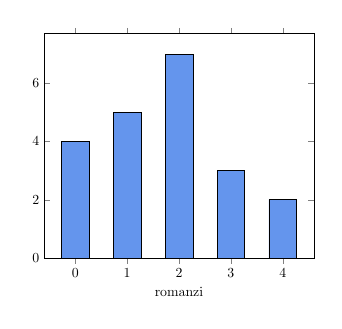
\begin{tikzpicture}[scale=.5]
\begin{axis}[ymin=0,
ybar,
xlabel=romanzi,
bar width=20pt,enlarge x limits=0.15
]
    \addplot[fill=CornflowerBlue,draw=black]
      coordinates{
(0,4)
(1,5)
(2,7)
(3,3)
(4,2)
      };
\end{axis}
\end{tikzpicture}
\end{center}
\end{esercizio}
\end{multicols}

\begin{esercizio}[Prove Invalsi~2004-2005]
\label{ese:A.58}
Il Ministero dell'Istruzione ha diffuso le seguenti informazioni sul numero 
di alunni stranieri della scuola italiana
nell'anno scolastico~2003-2004. La tabella riporta solo le~5 nazionalità 
più numerose.
\begin{center}
 \begin{tabularx}{.9\textwidth}{*{3}{X}}
\toprule
Nazionalità più numerose & Numero di alunni & Percentuale di alunni sul 
totale degli stranieri \\
\midrule
Albania & 50.000 & 18,00\% \\
Marocco & 42.000 & 15,00\% \\
Romania & 28.000 & 10,00\% \\
Cina & 16.000 & 6,00\% \\
Ecuador & 11.000 & 4,00\% \\
\bottomrule
\end{tabularx}
\end{center}

Cosa si può dedurre da tali dati sugli alunni stranieri di nazionalità 
russa? Sono~$\ldots$
\begin{multicols}{2}
\begin{enumeratea}
 \item meno di~11\,000;
 \item sicuramente meno di~400;
 \item fra il~4\% e il~18\%;
 \item assenti dalle scuole italiane.
\end{enumeratea}
\end{multicols}
\end{esercizio}

\begin{esercizio}[Prove Invalsi~2005-2006]
\label{ese:A.53}
In una classe di~25 alunni, i punteggi (abbreviati in tabella con~$p$) 
ottenuti in un test di matematica risultano distribuiti come indicato nella 
seguente tabella.
\begin{center}
 \begin{tabular}{l*{5}{c}}
\toprule
Punteggio & $0 \leq p < 20$ & $20 \leq p < 40$ & $40 \leq p < 60$ & $60 
\leq p < 80$ & $80 \leq p \leq~100$ \\
Numero alunni & & & & & \\
\bottomrule
\end{tabular}
\end{center}
Qual è la percentuale di alunni che ha ottenuto un punteggio inferiore a~60?
\end{esercizio}

\begin{esercizio}[Prove Invalsi~2005-2006]
\label{ese:A.54}
Un impiegato ha percepito per i primi~3 mesi dell'anno uno stipendio 
mensile di~850\officialeuro . Nei~9 mesi successivi ha percepito
lo stipendio mensile precedente aumentato di~200\officialeuro . Quant'è lo 
stipendio medio nell'anno di quell'impiegato?
\end{esercizio}

\begin{multicols}{2}
\begin{esercizio}[Prove Invalsi~2005-2006]
\label{ese:A.55}
Nel grafico seguente si riporta l'età dei ragazzi che frequentano una 
palestra. Qual è la media aritmetica dell'età dei ragazzi
se la distribuzione di frequenza è quella indicata nel grafico?
\begin{center}
 % (c) 2012 Dimitrios Vrettos - d.vrettos@gmail.com
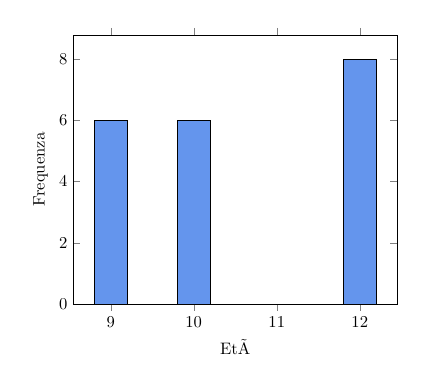
\begin{tikzpicture}[scale=.6]

\begin{axis}[ymin=0,
ybar,
ylabel=Frequenza,
xlabel=Età,
bar width=20pt,
enlarge x limits=0.15,]

\addplot[fill=CornflowerBlue,draw=black]
      coordinates{
	(9, 6)
	(10,6)
	(12,8) };
\end{axis}
\end{tikzpicture}

\end{center}
\end{esercizio}
\end{multicols}

\begin{multicols}{2}
\begin{esercizio}[Prove Invalsi~2006-2007]
\label{ese:A.56}
I~25 alunni della terza~$C$, dopo aver raccolto i voti conseguiti
nella verifica scritta di matematica, hanno costruito il seguente grafico:
Quanti ragazzi hanno conseguito come voto~7?

a)~12; \quad b)~7; \quad c)~5; \quad d)~3.
\begin{center}
 % (c) 2012 Dimitrios Vrettos - d.vrettos@gmail.com


\begin{tikzpicture}[x=10mm,y=10mm, x radius=10mm, y radius=10mm]
  \draw (0,0) circle (3);
  \draw[fill=orange] (0,0) -- (0:3) arc (0:14.4:3);
 \draw[fill=brown] (0,0)-- (14.4:3) arc (14.4:57.6:3);
 \draw[fill=green] (0,0)-- (57.6:3) arc (57.6:158.4:3);
\draw[fill=red] (0,0)-- (158.4:3) arc (158.4:273.6:3);
 \draw[fill=blue] (0,0)-- (273.6:3) arc (273.6:316.8:3);
 \draw[fill=olive] (0,0)-- (316.8:3) arc (316.8:345.6:3);
 \draw[fill=lightgray] (0,0)-- (345.6:3) arc (345.6:360:3);

\node[above]  at (0,3) {Voti di Matematica della classe terza $C$};
\begin{scope}[xshift=50mm,
every node/.style={ anchor=center}]
\matrix[matrix of nodes] at (0,0){
\node[fill=orange]{};&Voto 3\\
\node[fill=brown]{};&Voto 4\\
\node[fill=green]{};&Voto 5\\
\node[fill=red]{};&Voto 6\\
\node[fill=blue]{};&Voto 7\\
\node[fill=olive]{};&Voto 8\\
\node[fill=lightgray]{};&Voto 9\\
};
\end{scope}
\begin{scope}[every node/.style={rounded corners, fill=white, draw=black, font=\small}]
\draw(7.2:2.5) node {$4\%$};
\draw(36:2.5) node {$12\%$};
\draw(108:2.5) node {$28\%$};
\draw(216:2.5) node {$32\%$};
\draw(295.2:2.5) node {$12\%$};
\draw(331.2:2.5) node {$8\%$};
\draw(352.8:2.5) node {$4\%$};
\draw(7.2:2.5) node {$4\%$};
\draw(7.2:2.5) node {$4\%$};
\end{scope}
\end{tikzpicture}
\end{center}
\end{esercizio}
\end{multicols}

\begin{esercizio}
\label{ese:A.59}
La tabella mostra la superficie delle varie province del Lazio.
\begin{center}
 \begin{tabular}{l*{5}{c}}
 \toprule
 Provincia & Frosinone & Latina & Rieti & Roma & Viterbo\\
 Superficie ($\unit{km}^2$) & 3240& 2251& 2749& 5352& 3612\\
 \bottomrule
 \end{tabular}
\end{center}
Quale dei diagrammi riportati sotto descrive graficamente i dati della 
tabella?
\begin{center}
 % (c) 2012 Dimitrios Vrettos - d.vrettos@gmail.com


\begin{tikzpicture}[scale=.4,x=7mm,y=7mm]
  \draw (0,0) circle (3);
   \draw[fill=orange] (0,0) -- (0:3) arc (0:90:3);
 \draw[fill=brown] (0,0)-- (90:3) arc (90:133.2:3);
  \draw[fill=green] (0,0)-- (133.2:3) arc (133.2:198:3);
\draw[fill=red] (0,0)-- (198:3) arc (198:259.2:3);
\draw[fill=blue] (0,0)-- (259.2:3) arc (259.2:360:3);
\node[above] at (0,3) {1};

\begin{scope}[xshift=50mm]
  \draw (0,0) circle (3);
   \draw[fill=orange] (0,0) -- (0:3) arc (0:36:3);
 \draw[fill=brown] (0,0)-- (36:3) arc (36:64.8:3);
  \draw[fill=green] (0,0)-- (64.8:3) arc (64.8:180:3);
\draw[fill=red] (0,0)-- (180:3) arc (180:324.2:3);
\draw[fill=blue] (0,0)-- (324:3) arc (324:360:3);
\node[above] at (0,3) {2};
\end{scope}

\begin{scope}[xshift=100mm]
  \draw (0,0) circle (3);
   \draw[fill=orange] (0,0) -- (0:3) arc (0:39.6:3);
 \draw[fill=brown] (0,0)-- (39.6:3) arc (39.6:122.4:3);
  \draw[fill=green] (0,0)-- (122.4:3) arc (122.4:194.4:3);
\draw[fill=red] (0,0)-- (194.4:3) arc (194.4:309.6:3);
\draw[fill=blue] (0,0)-- (309.6:3) arc (309.6:360:3);
\node[above] at (0,3) {3};
\end{scope}


\begin{scope}[xshift=25mm, yshift=-50mm]
  \draw (0,0) circle (3);
   \draw[fill=orange] (0,0) -- (0:3) arc (0:68.4:3);
 \draw[fill=brown] (0,0)-- (68.4:3) arc (68.4:115.2:3);
  \draw[fill=green] (0,0)-- (115.2:3) arc (115.2:172.8:3);
\draw[fill=red] (0,0)-- (172.8:3) arc (172.8:284.4:3);
\draw[fill=blue] (0,0)-- (284.4:3) arc (284.4:360:3);
\node[above] at (0,3) {4};
\end{scope}

\begin{scope}[xshift=75mm, yshift=-50mm]
  \draw (0,0) circle (3);
   \draw[fill=orange] (0,0) -- (0:3) arc (0:126:3);
 \draw[fill=brown] (0,0)-- (126:3) arc (126:201.6:3);
  \draw[fill=green] (0,0)-- (201.6:3) arc (201.6:230.4:3);
\draw[fill=red] (0,0)-- (230.4:3) arc (230.4:304.4:3);
\draw[fill=blue] (0,0)-- (304.4:3) arc (304.4:360:3);
\node[above] at (0,3) {5};
\end{scope}

\begin{scope}[xshift=50mm, yshift=35mm]
\matrix[matrix of nodes, every node/.style={anchor=center}]{
\node[fill=orange]{};&Frosinone&
\node[fill=brown]{};&Latina&
\node[fill=green]{};&Rieti&
\node[fill=red]{};&Roma&
\node[fill=blue]{};&Viterbo\\};

\end{scope}
\end{tikzpicture}
\end{center}

\end{esercizio}

\begin{esercizio}[Prove Invalsi~2011]
\label{ese:A.48}
Il reddito medio annuo dei lavoratori agricoli di un certo paese ammonta 
a~3500 scudi e quello dei lavoratori dell'industria
a~4500 scudi. È corretto affermare che il reddito medio complessivo ammonta 
a~4000 scudi?
\end{esercizio}

\begin{esercizio}[\Ast Prove Invalsi~2011]
\label{ese:A.49}
La settimana scorsa la mamma chiese ad Aurelia di trascrivere al computer 
un manoscritto e Aurelia le assicurò che avrebbe
battuto~20 pagine al giorno. Per la prima metà del manoscritto andò 
piuttosto lentamente battendo~10 pagine al giorno e poi,
per recuperare il tempo perduto, trascrisse la seconda metà a~30 pagine al 
giorno.
Quando ebbe finito portò a sua madre la trascrizione dicendole: Vedi, ho 
fatto una media di~20 pagine al giorno,
come ti avevo promesso. Infatti~$(10+30)/2=20$ Non è vero, replicò sua 
madre.
\hfill [15]
\end{esercizio}

\begin{multicols}{2}
\begin{esercizio}[\Ast Prove Invalsi~2011]
\label{ese:A.50}
In una indagine sullo stato di salute della popolazione sono state raccolte 
informazioni relative al peso e
alla statura di~1000 intervistati. Gli intervistati sono stati poi 
suddivisi in quattro gruppi,
come riportato nel grafico seguente. Quante sono le persone in sovrappeso?

\begin{enumeratea}
 \item Più di~500, ma meno di~600;
 \item più di~600;
 \item meno della somma delle persone sottopeso e obese;
 \item all'incirca tante quante sono le persone normopeso.
\end{enumeratea}
\begin{center}
 % (c) 2012 Dimitrios Vrettos - d.vrettos@gmail.com

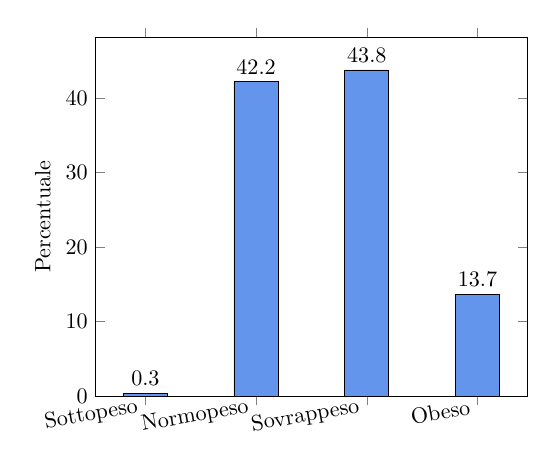
\begin{tikzpicture}[scale=.8]
\begin{axis}[ymin=0,
ybar,
xtick=data,
ylabel=Percentuale,
x tick label style={rotate=10,anchor=east},
symbolic x coords={Sottopeso, Normopeso, Sovrappeso, Obeso},
bar width=20pt,enlarge x limits=0.15,nodes near coords,
nodes near coords align={vertical},
]
    \addplot[fill=CornflowerBlue,draw=black]
      coordinates{
	(Sottopeso, .3)
(Normopeso, 42.2)
(Sovrappeso, 43.8)
(Obeso,13.7)
      };
\end{axis}
\end{tikzpicture}

\end{center}
\hfill [d]
\end{esercizio}
\end{multicols}

% \begin{esercizio}[Prove Invalsi~2004-2005]
% \label{ese:A.52}
% La seguente tabella si riferisce alla rilevazione effettuata in una classe 
% prima di un Istituto Tecnico.
% \begin{center}
%  \begin{tabular}{l*{4}{c}}
% \toprule
%  & \multicolumn{4}{c}{Scuola media di provenienza}\\
% Sesso & Scuola A & Scuola B & Scuola C & Altre scuole\\
% \midrule
% Maschi & 5 & 3 & 4 & 2 \\
% Femmine & 6 & 3 & 4 & 3 \\
% \bottomrule
% \end{tabular}
% \end{center}
% Qual è la percentuale di alunni provenienti dalla Scuola B?
% \end{esercizio}

